
%%%%%%%%%%%%%%%%%%%%%%%%%%%
\section{A list of books}
  
A list of books I like about general knowledge in science:

\begin{itemize}
\item[$\bullet$] L'aventure des nombres, Godefroy
\item[$\bullet$] L'autobigraphie de Paul Levy, Laurent Schwartz, et Yuri Manin.
\item[$\bullet$] Recoltes et semailles, Grothendieck.
\item[$\bullet$] Lee Smolin, The trouble with physics, the rise of String theory, the fall of a Science, and what comes next,
\item[$\bullet$] Julian Barbour, The End of Time, The next revolution in Physics,
\item[$\bullet$] Carlo Rovelli, Et si le temps n'existait pas, un peu de science subversive,
\item[$\bullet$] Mandlebrot, The (Mis)Behaviour of markets, Fractals and Chaos, the Mandelbrot set and beyond, The fractal geometry of nature.
\item[$\bullet$] Manjit Kumar:
\item[$\bullet$] Amir Alexander, Infinitesimal: How a Dangerous Mathematical Theory Shaped the Modern World
\item[$\bullet$] Ian Stewart, Does God play dice?
\item[$\bullet$] History of Statistics, Stielger
\item[$\bullet$] Logicomix\\
\end{itemize}

Overview and more specialized books:
\begin{itemize}
\item[$\bullet$] Moonshine beyond the Monster, Terry Gannon
\item[$\bullet$] Le theoreme d'uniformisation, Saint-Gervais
\item[$\bullet$] Invitation aux mathematiques de Fermat, Hellgouarch
\item[$\bullet$] Rached Mneime, tous ses livres!
\item[$\bullet$] Hubbard West pour les equa diff
\item[$\bullet$] Noether's theorem, Yvette K
\item[$\bullet$] Nother's wonderful theorem
\item[$\bullet$] The annus mirabellus of Einstein
\item[$\bullet$] The Road to Reality, Sir Roger Penrose \\
\end{itemize}

Books about Einstein: 
\begin{itemize}
\item[$\bullet$] Subtle is the Lord, Abraham Pais \cite{Pais1982}; biography of Einstein by someone who knew him;
\item[$\bullet$] Einstein's miraculous year: Five papers that changed the face of physics, Penrose \& Einstein \cite{Penrose2005Einstein}; English translations of the five papers Einstein published in 1905 while working at the patent office in Bern.  
\item[$\bullet$] Quantum: Einstein, Bohr, and the great debate about the nature of reality, Kumar \cite{Kumar}; history of quantum theory from Planck's blackbody radiation to the EPR paradox.
\end{itemize}
%%%%%%%%%%%%%%%%%%%%%%%%
\section{Seminar}

%%%%%%%%%%%%%%%%%%%%%%%%%%%%%%%%
\subsection{Cartan subalgebras}
%%%%%%%%%%%%%%%%%%%%%%%%%%%%%%%%

Out of any inclusion of $C^*$-algebras $A\subseteq B$ with $A$ unital commutative, we construct an action of the normalizer of $A$ in $B$ by partial homeomorphism on $X$ the spectrum of $A$, i.e. a homomorphism of semigroup  
\[\alpha: N_B(A) \rightarrow SHomeo(X).\] 

If $n\in N_B(A)$ and $x\in Spec(A)$, set 
\[\langle \alpha_n(x) , a\rangle =\langle x , n^*a n\rangle .\]
This defines a homeomorphism 
\[\alpha_n : U_n \rightarrow U_{n^*},\]
where $U_n = \{x\in Spec(A), n^*n(x) >0\}$ such that $\alpha_{nm} =\alpha_{n} \circ \alpha_{m}$.\\
 
If $A$ is maximal abelian in $B$, and other conditions, then $B$ is shown to be isomorphic to the twisted reduced $C^*$-algebra of the groupoid of stalks of $N_B(A)$. This can be seen  as an extension of the Gelfand transform
\[\left\{\begin{array}{rcl}
B & \rightarrow & C^*_r(G) \\
b & \mapsto &  \\
\end{array}\right.\] 

%%%%%%%%%%%%%%%%%%%%%%%%%%%%%
\subsection{Dynamical Property (T)}
%%%%%%%%%%%%%%%%%%%%%%%%%%%%%

The first thing I will try to do is to justify the use of groupoids. My opinion is that these objects are not loved as much as they deserve. People who very much like short and concise definitions enjoy to say that \textit{groupoids are small categories in which all morphisms are invertible.} This is true, but maybe does not shed light on the reasons people look at such objects. \\

Groupoids can be thought as a generalisation of both groups and spaces. In that effect, a groupoid $G$ is made of two parts, in our case, two spaces, the \textit{group-like} part $G$ and the \textit{space-like} part $G^0$. Usually $G$ is called the space of arrows, and $G^0$ the base space, seen as a subset of $G$. Any arrow $g\in G$ has a starting point $x\in G^0$ and an ending point $y\in G^0$. This is encoded by two maps $s,r : G \rightrightarrows G^0$ called source and range. Two arrows can be composed as long as the ending point of the first coincides with the starting point of the second. The points of the base space act as units, and every arrow as an inverse with respect to this partial multiplication.

\[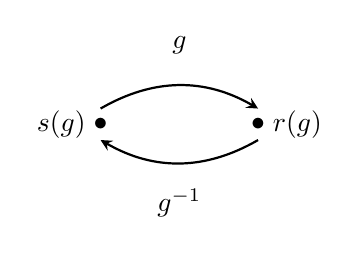
\begin{tikzpicture}
\draw  (0,1) node {$g$};
\draw  (0,-1) node {$g^{-1}$};
\draw [>=stealth, ->, thick] (-1,0.2) to[bend left] (1,0.2);
\draw [>=stealth, ->,thick] (1,-0.2) to[bend left] (-1,-0.2);
\draw  (-1,0) node {$\bullet$};
\draw  (-1.5,0) node {$s(g)$};
\draw  (1,0) node {$\bullet$};
\draw  (1.5,0) node {$r(g)$};
\end{tikzpicture}\]

In our setting, all the spaces will be topological spaces and the maps will be continuous. We will even simplify greatly our life by only looking at second countable, locally compact, étale groupoids with compact base space. From now on, we will only say \textit{étale}, forgetting about all other technical assumptions to gain in clarity.\\ 

Being étale means that the range map $r: G \rightarrow G^0$ is a local homeomorphism, i.e. for every $g\in G$, there exists a neighborhood $U$ of $g$ such that $r_{|U}$ is a homeomorphism. This implies in particular that every fiber $G^x = r^{-1}(x)$ and $G_x = s^{-1}(x)$ are discrete. When the base space $G^0$ has the additional property of being totally disconnected, we will say that $G$ is \textit{ample}. Here is a list of examples of étale groupoids.\\

\begin{itemize}
\item[$\bullet$] A (nice) compact space $X$ defines a trivial groupoid $G=G^0=X$ and source and target are the identity; in the opposite direction if the base space is a point, the groupoid is a group. One can already see how the notion of groupoid generalises both spaces and groups as promised.  \\

\item[$\bullet$] As an intermediate situation between these two cases, consider a discrete group $\Gamma$ acting by homeomorphisms on a compact space $X$. Define the \textit{action groupoid} as follow. Topologically, it is the space $G= X\times \Gamma \rightrightarrows G^0 = X$. The multiplication encodes the action
\[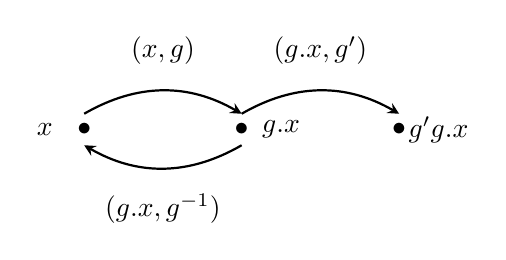
\begin{tikzpicture}
\draw  (0,1) node {$(x,g)$};
\draw  (0,-1) node {$(g.x,g^{-1})$};
\draw  (2,1) node {$(g.x,g')$};
\draw [>=stealth, ->, thick] (-1,0.2) to[bend left] (1,0.2);
\draw [>=stealth, ->,thick] (1,-0.2) to[bend left] (-1,-0.2);
\draw [>=stealth, ->, thick] (1,0.2) to[bend left] (3,0.2);
\draw  (-1,0) node {$\bullet$};
\draw  (-1.5,0) node {$x$};
\draw  (1,0) node {$\bullet$};
\draw  (1.5,0) node {$g.x$};
\draw  (3,0) node {$\bullet$};
\draw  (3.5,0) node {$g'g.x$};
\end{tikzpicture}\]
and this picture gives every element to reconstruct the groupoid.\\

\item[$\bullet$] If $R\subseteq X\times X $ is an equivalence relation, then $R$ as a canonical structure of groupoid with the base space being the diagonal $R^0 = \{ (x,x) \ | \ x\in X\}$ and the multiplication being the only one possible
\[(x,y)(y,z) = (x,z).\] 

\item[$\bullet$] More interesting is the \textit{coarse groupoid} $G(X)$ associated to a discrete countable metric space $(X,d)$ with bounded geometry, that is
\[\sup_{x\in X} |B(x,R)| < \infty \quad \forall R>0.\]
A nice way of thinking about this condition is to imagine yourself looking at the space with a magnifying glass of prescribed radius, but as great as you wish. Then you should not observe more and more points in your sight as you move around. In other words, the points fitting in the radius of your glass is uniformly bounded.\\

Now consider the $R$-diagonals:
\[\Delta_R = \{(x,y) \ | \ d(x,y) < \infty\}\subseteq X\times X\]
and take their closure $\overline{\Delta_R }$ in $\beta (X\times X) $ ($\beta Y$ being the Stone-\v{C}ech compactification of $Y$). The coarse groupoid is defined topologically as 
\[G(X) = \cup_{R>0} \overline{\Delta_R} \rightrightarrows \beta X ,\]
and is endowed with the structure of an \textit{ample} groupoid which extend the groupoid $X\times X \rightrightarrows X$ associated with the coarsest equivalence relation on $X$. The topological property of this groupoid encodes the metric or \textit{coarse} property of the space. For instance, $X$ has property A iff $G(X)$ is amenable, $X$ is coarsely embeddable into a Hilbert space iff $G(X)$ has Haagerup's property, etc.\\
\item[$\bullet$] The last construction is associated to what is often referred as an \textit{approximated group}, which is the data of $\mathcal N = \{ \Gamma , \{N_k\}\}$ where $\Gamma$ is a discrete group, and the $N_k$'s are a tower of finite index normal subgroups with trivial intersection, i.e. 
\[N_1 \triangleleft N_2 \triangleleft ... \quad \text{s.t. } \cap_k N_k = \{ e_\Gamma\} \text{ and } [\Gamma	: N_k] < \infty.  \]
Then the $\Gamma_k$'s are finite groups. Set $\Gamma_\infty = \Gamma$ for convenience (which is not usually finite!). For any discrete group $\Lambda$, there exists a left-invariant proper metric, which is unique up to coarse equivalence (take any word metric if the group is finitely generated). Let us denote by $|\Lambda |$ the coarse class thus obtained. Then the first object of interest in that case is the coarse space $X_\mathcal{N}$ defined as the \textit{coarse disjoint union}
\[X_\mathcal{N} = \coprod_k |\Gamma_k |.\]
Here the metric is such that $d(| \Gamma_i| , |\Gamma_j| )\rightarrow \infty $ as $i+j$ goes to $\infty$, $i\neq j$.\\

The second interesting object attached to $\mathcal{N}$ is the HLS (after Higson-Lafforgue-Skandalis \cite{HLS}, where it was first defined to build counter-examples to the Baum-Connes conjecture) groupoid. The base space is the Alexandrov compactification  of the integers 
\[G_\mathcal{N}^0 = \overline{\N},\]
and $G_\mathcal{N}$ is a bundle of groups with the fiber of $k$ being $\Gamma_k$. The topology is taken to be discrete over the finite base points, and a basis of neighborhood of $(\infty,\gamma)$ is given by 
\[\mathcal{V}_{\gamma, N} = \{(k, q_k(\gamma)) \ | \ k\geq N \} \quad N\in\N ,\]
where $q_k : \Gamma \rightarrow \Gamma_k$ is the quotient map.\\
 \end{itemize}

One of the reasons we use groupoids is that they are convenient to build interesting $C^*$-algebras. To see their relevance, one may start with the question \textit{What are operator algebraists doing?} A possible answer is that part of Noncommutative Geometry and Operator Algebras are devoted to the construction of interesting classes of $C^*$-algebras. For instance, \textit{nuclearity} was naturally introduced after Grothendieck's work, followed by a $C^*$-algebraic formulation. Arises then the question \textit{does there exist nonnuclear $C^*$-algebras?} A now classical result states that, when $\Gamma$ is a discrete group, the reduced $C_r^*(\Gamma)$ is nuclear iff $\Gamma$ is amenable. Calling out a nonamenable group, like any nonabelian free group, produces then a nonnuclear $C^*$-algebra. This game revealed itself to be very fruitful: study a property in some field and try to apply it to $C^*$-algebras to see what exotic being can be built out of it. The most common fields that have natural $C^*$-algbras associated to them are traditionally group theory, coarse geometry and dynamical systems (there are others like foliations etc, but let me just limit myself to these ones). This can be summarized in the following diagram.

%%%%%%%%%%%%%%%%%%%%%%%%%%%%%%%%%%%%%%%%%%%%%%%%%%%%%%%%%%%%%%%%%%%%%%%%%%%
\[\begin{tikzpicture}[node distance=1cm, auto,]
 %nodes
\node[punkt] (C) {$C^*$-algebras};\\
\node[punkt, above=of C] (G) {Groupoids};
\node[above=of G] (dummy) {};
\node[punkt, right=of dummy] (CG) {Coarse Geometry}
	edge[pil, bend left=45] node[auto] {$G(X)$} (G.east); 
\node[punkt, left=of dummy] (TD) {Topological dynamics}
	edge[pil, bend right=45] node[auto] [below left] {$\Omega\rtimes \Gamma$} (G.west); 
\node[punkt, above=of dummy] (GT) {Group theory}
	edge[pil, bend left=45] node[auto] {$Cay(\Gamma,S)$} (CG.north) 
	edge[pil, bend right=45] node[auto] [above left] {$\Gamma \curvearrowright \Omega$} (TD.north);

\draw[vecArrow] (G) to (C);
\end{tikzpicture}\]
%%%%%%%%%%%%%%%%%%%%%%%%%%%%%%%%%%%%%%%%%%%%%%%%%%%%%%%%%%%%%%%%%%%%%%%%%%%

Another interesting strategy is to try and translate a property in one of those upper boxes directly in terms of groupoids. Then the property can either be used to build $C^*$-algebras, either give a new definition in the case of other upper boxes. For instance, that is what we tried to do with Rufus Willett in our work on property T. Property T is originally a group property defined in terms of its unitary representations. In \cite{WillettYu}, Willett and Yu defined a geometric property T for monogenic discrete metric spaces with bounded geometry. Following their work, our first goal was to try and define a property T for (nice enough) topological groupoids so that in the case of groups and coarse groupoids, it reduces to these notions of property T. It gives then a notion of property T for dynamical systems, by considering property T for the action groupoid $X\rtimes \Gamma$. The second part of the work is dedicated to go down the last arrow, that is studying implications of property T for $G$ to its reduced and maximal $C^*$-algebras, and even more general completions of $C_c(G)$.\\

Let us first recall what is property T for discrete groups.\\

If $\pi : \Gamma \rightarrow B(H)$ is a unitary representation of $\Gamma$ on a separable Hilbert space, say that $\pi$ almost has invariant vectors if for every pair $(F,\varepsilon)$ where $F$ is a finite subset of the group and $\varepsilon$ a positive number, there exists a unit vector $\xi\in H$ such that 
\[ \| s.\xi - \xi \| < \varepsilon\quad \forall s\in F. \]
\begin{definition}
A group $\Gamma$ has property T if every representation that almost has invariant vectors admits a nonzero invariant vector.
\end{definition}

This definition is not the original one. Indeed property T was defined by Kazhdan in order to prove that \textit{some} lattices in \textit{some} Lie groups were finitely generated. It seemed a very specific property and application, but it turned out that property T gave very nice applications. Here are some of the most spectacular the author is aware of.\\

\begin{itemize}
\item[$\bullet$] Margulis supperrigidity theorem (about this, see Monod's \cite{MonodSuperrigidity} beautiful generalization, which Erik called the most beautiful paper he ever read);\\
\item[$\bullet$] existence of expander: for any infinite approximated group (in the sense of the examples above) $\Gamma$, the space $X_\mathcal{N}$ is an expander;\\
\item[$\bullet$] existence of Kazdhan projections which are very wild objects one should only approach with care; \\
\item[$\bullet$] more generally, property T was for a long time an obstruction to the Baum-Connes conjecture, up until the work of Lafforgue (\cite{LafforgueHyperbolic}, \cite{Lafforgue}). It still gives interesting properties for diverse crossed-product constructions as we will see.\\ 
\end{itemize}

One can prove easily that finite groups have T. Indeed, in that case, take the finite subset to be the whole group and look intensely at the identity
\[ \| s.\xi - \xi \|^2 = 2 ( 1 - Re \langle s.\xi ,\xi \rangle ).  \]
If $\xi$ is $(\Gamma,\varepsilon)$-invariant for $\varepsilon$ sufficiently small, then the above identity implies that $\frac{1}{|\Gamma |} \sum_{s\in \Gamma} s.\xi $ is nonzero because its inner-product with $\xi$ will have real part close to $1$. But $\xi$ is invariant.\\

Now take $\Gamma = \Z$ and look at the left-regular representation, i.e. $H = l^2\Gamma$ and 
\[(s.\xi)(x) = \xi(s^{-1}x).\]
Then if $\xi_n = \frac{1}{|F_n|} \chi_{F_n}\in H$ is the characteristic function of $F_n$ normalized to be a unit vector, one can check that 
\[ \sup_{s\in F}\| s.\xi_n - \xi  \| \rightarrow 0 \text{ as }n\rightarrow \infty \]
so that the regular representation always almost has invariant vectors. But it never has nonzero invariant ones, so that $\Z$ does not have T. This proof actually works for every infinite amenable group. \\

The moral of this story is that if one wants to find infinite groups with property T, one has to look at nonamenable groups. Maybe $\mathbb F_2$ or $SL(2,\Z)$? Actually not: they both surject to $\Z$ which does not have T, and this is an obstruction to having T as is obvious from the definition.\\

Finding infinite groups with property T is actually a hard problem. Here are some examples, without any proofs since these would go out of scope for these notes.\\
\begin{itemize}
\item[$\bullet$] $SL(n,\R)$ and $SL(n,\Z)$ if $n\geq 3$;\\
\item[$\bullet$] $Sp(n,1)$ and its lattices, which gives examples of infinite hyperbolic (in the sense of Gromov) groups having property T;\\
\item[$\bullet$] $Aut(\mathbb{F}_5)$ and $Out(\mathbb{F}_5)$ by a recent result of Nowak and Ozawa \cite{NowakOzawa}. Their proof is interesting in that they use numerical computations to reach their result using a previous result of Ozawa \cite{OzawaT};\\
\item[$\bullet$] $SO(p,q)$ with $p> q \geq 2$ and $SO(p,p)$ with $p \geq 3$. More generally, any real Lie group with real rank at least two, and all their lattices. Also, any simple algebraic group over a local field of rank at least two have T.\\ 
\end{itemize} 

To define property T for groupoids, we need to choose what kind of representations we are looking at, and to decide what are the invariant vectors.\\

A representation will be a $*$-homomorphism $\pi : C_c(G)\rightarrow B(H)$. A vector $\xi\in H $ is called invariant if \[f.\xi = \Psi(f).\xi \quad \forall f\in C_c(G).\]
The subspace of invariant vectors is denoted by $H^\pi$ and its orthogonal complement, the space of coinvariants, is denoted by $H_\pi$.\\

Here $Psi$... Groups\\

Let $\mathcal{F}$ be a family of representations.
\begin{definition}
$G$ has property T if there exists a pair $(K,\varepsilon)$ where $K\subseteq G$ is compact and $\varepsilon>0$ such that, for every $\pi \in \mathcal{F}$, there exists $f\in C_K(G)$ such that $\| f\|_I \leq 1$ and 
\[\|f .\xi - \Psi (f).\xi \| < \varepsilon \| \xi\| \quad \forall \xi \in H_\pi. \]
\end{definition}
 
The first thing we did was to study what were the relationships between groupoid property T and other property T.\\

\begin{itemize}
\item[$\bullet$] if $G=\Gamma$ is a discrete group, $\Gamma$ has property T iff $G$ has property T (in the groupoid sense);\\
\item[$\bullet$] if $X$ is a coarsely geodesic metric space, then $X$ has geometric property T iff $G(X)$ has property T;\\
\item[$\bullet$] in the case of a topological action, $X\rtimes \Gamma$ has property T iff $\Gamma$ has T w.r.t. the family $\mathcal{F}_X$ of representations $\pi : \C[\Gamma]\rightarrow B(H) $ s.t. there exists a representation $\rho: C(X) \rightarrow B(H)$ such that $(\rho, \pi) $ is covariant. This hypothesis simplifies in the case where there exists a invariant ergodic probability measure on $X$; in that case property T for $X\rtimes \Gamma$ and for $\Gamma$ are equivalent;\\
\item[$\bullet$] in the case of an approximated group $\Gamma$, then $G_\mathcal{N}$ has property T iff $\Gamma$ has T. This may sound disappointing, but if one refines the result, one gets the nice following property: $\Gamma$ has property $\tau$ w.r.t. $\mathcal{N}$ iff $G_\mathcal{N}$ has T w.r.t. the family of representations that extend to the reduced $C^*$-algebra of $G$.\\
\end{itemize} 

The last part of the work is devoted to the existence of Kazdhan projections. Recall, if $\mathcal{F}
$ is a family of representations, $C^*_\mathcal{F}(G)$ is the $C^*$-algebra obtained as the completion of $C_c(G)$ w.r.t. the norm
\[\| a \|_\mathcal{F} = \sup_{\pi \in \mathcal{F}} \{ \| \pi(a) \|\}. \]
A Kazdhan projection $p\in C^*_\mathcal{F}(G)$ is a projection such that its image in any of the representations in $\mathcal{F}$ is the orthogonal projection on the invariant vectors.\\

\begin{thm}
Let $G$ be compactly generated. Then if $G$ has property T w.r.t. $\mathcal{F}$, there exists a Kazdhan projection $p\in C^*_\mathcal{F}(G)$. 
\end{thm}

This gives an obstruction to inner-exactness. Denote by $F$ the closed $G$-invariant subset 
\[\{x\in G^0 \ | \ G^x \text{ is infinite }\}\]
and $U$ its complement.\\

\begin{thm}
Let $G$ be compactly generated and with property T. If one can find a sequence of points $(x_i)_i\subset U$ such that, for every compact subset $K \subset G$, $K$ only intersects a finite number of orbits $G.x_i = r(s^{-1}(x_i))$, then $G$ is not inner-exact. In fact it is not $K$-inner-exact. in particular, at least one of the groupoids $G$, $G_{|U}$ or $G_{|U}$ does not satisfy the Baum-Connes conjecture.
\end{thm}

%%%%%%%%%%%%%%%%%%%%%%%%%%%%%%%%%%%%%%%%
\subsection{Classification and the UCT}
%%%%%%%%%%%%%%%%%%%%%%%%%%%%%%%%%%%%%%%%

For $A$ a simple unital $C^*$-algebra, the Elliot invariant is:
\[Ell(A) = \left( K_0(A), K_0(A)_+ , [1_A]_0 , K_1(A), T(A) , r_A : T(A) \rightarrow S(K_0(A)) \right) ,\]
here $T(A)$ is the trace space and $r_A$ the paring $r_A(\tau)([p]) = [\tau(p)]$.\\

\textbf{Elliot's conjecture:} Separable, simple, nuclear are classifiable by Elliot's invariants.

\begin{thm}
Separable, simple, unital, nuclear, $\mathcal Z$-stable, UCT algebras are classifiable by Elliot's invariants.
\end{thm}

An example of a classification theorem: Elliot's theorem,

\begin{thm}
Let $A$ and $B$ unital AF-algebras and \[\alpha : K_0(A) \rightarrow K_1(A)\]
a unital order isomorphism, i.e. \[\alpha(K_0(A)_+) \subseteq K_0(B)_+ \quad \text{and} \quad \alpha([1_A])=[1_B].\]
Then there exists a unital $*$-isomorphism $\phi; A\rightarrow B$ such that $\phi_*=\alpha$.
\end{thm}

\newpage
%%%%%%%%%%%%%%%%%%%%%%%%%%%%%
\subsection{$C^*$-simplicity}
%%%%%%%%%%%%%%%%%%%%%%%%%%%%%

We only consider discrete countable groups, usually denoted by $\Gamma$.

\begin{definition}
A group is said to be $C^*$-simple if its reduced $C^*$-algebra is simple, i.e. has no proper closed two sided ideals. 
\end{definition}

A motivation for the interest toward such a notion can be the following result of Murray and Von Neumman: the Von Neumman algebra $L(\Gamma)$ is simple (no proper weakly closed two sided ideals) iff it is a factor iff $\Gamma$ is ICC (infinite conjugacy classes, i.e. all non trivial conjugacy classes are infinite). Another one is that simplicity is one out of the 5 criteria (unital simple separable UCT with finite nuclear dimension) needed in the classification theorem obtained by Winter et. al.\\  

Recall that, given two unitary representations of $\Gamma$, we say that $\pi$ is weakly contained in $\sigma$ and write 
\[\pi < \sigma\]
if every positive type function associated to $\pi$ can be approximated uniformly on compact sets by finite sums of such things associated to $\sigma$. In other words, if for every $\xi \in H_\pi$, $F\subseteq \Gamma$ finite and every $\varepsilon >0$, there exists $ \eta_1, \eta_2, ... , \eta_k$ such that
\[ | \langle \pi(s)\xi, \xi\rangle - \sum_i \langle \sigma (s)\eta_i,\eta_i \rangle| < \varepsilon \quad \forall s\in F.\]

Remark: one can restricts to convex combinations of normalized positive type functions.\\ 

If $\pi < \sigma$, then the identity $\C [\Gamma] \rightarrow \C [\Gamma]$ extends to a surjective $*$-morphisms
\[C_\sigma^*(\Gamma) \rightarrow C_\pi^*(\Gamma).\]

Indeed, it suffices to show that for every $a\in \C [\Gamma]$, \[ \| \pi(a)\| \leq \| \sigma(a)\|. \]
As $\| \pi(a)\|^2 = \| \pi(a^*a)\|$, we can suppose $a$ positive. Then
\[\begin{split}
 \langle \pi(s)\xi, \xi\rangle  & \leq   \sum_i t_i \langle \sigma (s)\eta_i,\eta_i \rangle +\varepsilon \\
				& \leq \| \sigma(a)\|+ \varepsilon
\end{split}\]
hence $\| \pi(a)\| \leq \| \sigma(a)\| +\varepsilon$, and let just $\varepsilon $ go to zero.

\begin{definition}
A group $\Gamma$ is $C^*$-simple if its reduced $C^*$-algebra is simple (i.e. has no proper closed two sided ideal).
\end{definition}

\begin{thm}
If $\Gamma $ has a non trivial amenable normal subgroup, then it is not $C^*$-simple.
\end{thm}

\begin{dem}
Let $N$ be a normal amenable subgroup of $\Gamma$. Let $(F_k)$ be a sequence of Folner sets for $N$, and 
\[\xi_k =\frac{1}{|F_k|}\chi_{F_k}\in l^2(\Gamma)\]
Then
\[\langle \lambda_\Gamma(s)\xi_k, \xi_k\rangle = 2- \frac{|F_k \Delta sF_k |}{|F_k|} \]
wich is $0$ if $s\notin N$, and goes to $1$ as $n$ goes to infinity if $s\in N$. In other words
\[\langle \lambda_\Gamma(s)\xi_k, \xi_k\rangle \rightarrow \langle \lambda_{\Gamma/N}(s)\delta_{eN} , \delta_{eN} \rangle,\]
which shows that $\lambda_{\Gamma / N} < \lambda_\Gamma$. This gives us a surjective $*$-morphism 
\[\phi : C^*_r(\Gamma)\rightarrow C^*_{\Gamma/N}(\Gamma).\]

A faster way which still works out when the ambient group is only locally compact is to point out that, $N$ being amenable, 
\[1_N < \lambda_N,\]
ensures by induction 
\[Ind_N^\Gamma 1_N = \lambda_{\Gamma / N} < Ind_N^\Gamma \lambda_N= \lambda_{\Gamma }.\]

But if $n\in N$ is non trivial, $\lambda_{\Gamma}(n)$ is non trivial and sent to $\lambda_{\Gamma /N}(n) = 1$ via $\phi$, so that $Ker\ \phi$ is a proper ideal in $C^*_r(\Gamma)$.\\	
\qed	 
\end{dem}

After the talk, Erik Guentner suggested the following proof. It is even shorter and doesn't assume any knowledge about weak containment or induction of representations. It is a weakening of the following fact: when $\Gamma$ is amenable, the trivial representation $1_\Gamma : C^*_{max}(\Gamma)\rightarrow \C$ extends to the reduced $C^*$-algebra.\\

Indeed let $a\in \C [\Gamma]$ and $(F_n)$ be a sequence of Folner sets for the support of $a$. Define $\xi_n = \frac{1}{|F_n|^\frac{1}{2}} \chi_{F_n} \in l^2(\Gamma )$. Then, suppose $a$ is positive, and compute
\[\begin{split}
\langle a \xi_n , \xi_n \rangle & = \sum_{s\in \text{ supp }a} a_\gamma \frac{|F_n \cap sF_n|}{|F_n|} \\ 
				& \rightarrow \| a \|_{1_\Gamma}
\end{split}\]
so that $ \| a\|_r \leq \| a\|_{1_\Gamma} $.\\

Now if $N$ is a normal amenable subgroup of $\Gamma$...\\

We saw that $\mathbb F_2$ is $C^*$-simple, yet it has a copy of $\Z$ as an amenable subgroup (non normal), and a normal (non amenable) subgroup: the commutator subgroup, which is an infinite rank free group, $\langle [x,y ] : x,y \in \mathbb F_2\rangle = \mathbb F([a^n, b^m] ; n,m) $. Both conditions are necessary.\\

This result led to following (false) conjecture: a group is $C^*$-simple iff it has no non trivial amenable normal subgroups.\\

\subsection{Completely positive maps}

If $A$ and $B$ are $C^*$-algebra, then a linear map $\phi : A\rightarrow B$ is called completely positive if 
\[\phi^{(n)}(a) = (\phi(a_{ij}))_{ij} \geq 0 \quad \forall a \in M_n(A)_+.\]
Denote $CP(A,B)$ the normed vector space of completely positive maps form $A$ to $B$. $S(A)$ denotes the state space of $A$, endowed with the weak-$*$ topology (it's then a convex subspace of $A^*$, compact when $A$ is unital).\\

Then: \\
\begin{itemize}
\item[$\bullet$] $CP(C(X),C(Y)) \cong C(Y, P(X))$ via $\mu_y(f) = \Phi(f)(y)$; \\

\item[$\bullet$] $CP(A,C(Y)) \cong C(Y, S(A))$ via $\omega_y(f) = \Phi(a)(y)$;\\

\item[$\bullet$] What about $CP(C(X),B)$? Continuous sections on the continuous field of $C^*$-algebras $\bigoplus_{\omega\in S(B)} B(H_\omega)$.\\
\end{itemize}

\subsection{Dynamical characterization of $C^*$-simplicity}
(Facts we are using: \\ 
$C(\partial_F \Gamma)$ is $\Gamma$-injective, in particular any $\Gamma$-equivariant u.c.p. $C(\partial_f \Gamma)\rightarrow A$ is spit, so is an isometric embedding,\\
$\partial_F \Gamma$ is totally disconnected, ) \\

The goal of this section is to prove the following theorem.

\begin{thm}
$\Gamma$ is $C^*$-simple iff the action of $\Gamma$ on $\partial_F \Gamma$ is free.
\end{thm}

Let's do first the forward direction.\\

Suppose the action is free. First, to show $C^*_r(\Gamma)$ is simple, it is enough to show that any representation 
\[\pi : C^*_r(\Gamma) \rightarrow B(H) \]
is injective. \\

By Arveson's extension theorem, $\pi$ extends to a u.c.p. map 
\[ \phi : C(\partial_F \Gamma)\rtimes_r \Gamma \rightarrow B(H). \]
Its restriction $\phi_0$ to $C(\partial_F \Gamma)$ is $\Gamma$-equivariant, because $C(\partial_F \Gamma)$ is in the multiplicative domain of $\phi_0$, and thus must be an isometric embedding, by $\Gamma$-injectivity of $C(\partial_F \Gamma)$ (it is split because $\C \subseteq B(H)$). The equivariant u.c.p. map $\phi_0$ is an isomorphism onto its image: extend its inverse form $im \  \phi_0$ to $im \ \phi$ and denote the resulting u.c.p map by $\tau$. \\

Claim: $\Psi = \tau \circ \phi $ is the canonical expectation $E : C(\partial_F \Gamma)\rtimes_r \Gamma \rightarrow C(\partial_F \Gamma)$ which is faithful. This implies $\pi$ is injective.\\

Let's end up with the claim. 
\begin{itemize}
\item[$\bullet$] $\Psi_{|C(\partial_F \Gamma)} = id_{C(\partial_F \Gamma)}$. Indeed, $\tau$ is the inverse of $\phi_0 = \phi_{C(\partial_F \Gamma)}$.
\item[$\bullet$] If $\gamma\neq e_\Gamma$, the action being free, for every $x$ there exists a function $f\in C(\partial_F \Gamma)$ such that 
\[f(x)\neq 0 \quad \text{and} \quad f(s^{-1}x) =0.\]
Now $C(\partial_F \Gamma)$ is in the multiplicative domain of $\Psi$, so
\[ \Psi(\lambda_s) f = \Psi( \lambda_s f) = \Psi( (sf)\lambda_s ) = (sf) \Psi( \lambda_s ) \]
which evaluated at $x$ gives $\Psi(\lambda_s)(x) = 0$, for all $x$, so $\Psi(\lambda_s)=0$. \\ 
\end{itemize}

The other direction is more intricated. It consists in two steps:\\
\begin{enumerate}
\item if $x\in \partial_F \Gamma$, then the stabilizer $\Gamma_x$ is amenable, which implies that $\lambda_{\Gamma/ \Gamma_x} <  \lambda_{\Gamma}$,\\
\item if $X$ is a $X$ is a $\Gamma$-boundary, and $\gamma\neq 0$ such that $int(X_s)\neq \emptyset$, then $\lambda_{\Gamma} \nless \lambda_{\Gamma/ \Gamma_x}  $, so that the kernel of $C^*_r(\Gamma)\rightarrow C^*_{\lambda_{\Gamma/ \Gamma_x}}(\Gamma)$ is a non trivial two sided closed ideal.\\
\end{enumerate}
This, together with the fact that $\partial_F\Gamma$ is topologically free iff it is free, concludes the proof.\\

First bullet: \\

\begin{itemize}
\item[$\bullet$] there exists a $\Gamma_x$-equivariant injective $*$-homomorphism
\[ \rho:  l^\infty (\Gamma_x ) \rightarrow l^\infty (\Gamma)\]
defined by $\rho(f)(ts_i)= f(t)$ for every $t\in\Gamma_x $, $\{s_i\}_i$ being a system of representatives of the right cosets $\Gamma_x \backslash \Gamma$.\\
\item[$\bullet$] there exists a $\Gamma_x$-equivariant u.c.p. map \[\psi : l^{\infty } \rightarrow C(\partial_F \Gamma),\] by universal property of $\partial_F \Gamma$, and the fact that the spectrum of $l^\infty(\Gamma)$ is $\beta \Gamma$. (for any compact $\Gamma$-space, there exists a $\Gamma$-map $\partial_F \Gamma \rightarrow P(X)$. take the dual of this map for $X = \beta \Gamma$).\\

\item[$\bullet$] The composition $\phi = ev_x \circ \psi \circ \rho$ defines a $\Gamma_x$-invariant state on $l^\infty(\Gamma_x)$, which concludes the proof.\\
\end{itemize}

Second bullet:\\

This needs a lemma:

\begin{lem} Let $X$ be a $\Gamma$-boundary.
For every non empty subset of $X$, every $\varepsilon >0$, there exists a finite subset $F\subset \Gamma \backslash \{e_\Gamma\}$ such that
\[ \min_{t\in F} \mu(tU^c) <\varepsilon \quad \forall \mu \in P(X).	 \]
\end{lem}

\begin{proof} 
Let $x\in U$. By strong proximality, there exists $t_\mu \neq e_\Gamma$ such that
\[\delta_x(U) - \mu(t_\mu U) = \mu(t_\mu U^c)<\varepsilon,\]
and by continuity of the action 
\[V_\mu = \{\nu\in P(X)\ | \ \nu(t_\mu U^c)< \varepsilon \}\]
is a neighboorhood of $\mu$. By compactness of $P(X)$ in the weak-$*$ topology, we can extract a finite cover such that 
\[P(X) = \cup_{i=1,m} V_{\mu_i}.\]
Then $F= \{ t_{\mu_1}, ..., t_{\mu_m}\}$ fills the requirements of the lemma.\\ 
\end{proof}

Suppose the action is not topologically free and let $s\neq e_\Gamma$ such that the interior $U$ of $X_s$ is not empty. Let $F$ the finite subset given by the lemma for $U$ and $\varepsilon = \frac{1}{3}$. Suppose 
\[\lambda_{\Gamma} < \lambda_{\Gamma / \Gamma_x}.\]
We will show this is absurd by looking at the coefficient $c_\gamma=\langle \lambda_\Gamma (\gamma)\delta_e , \delta_e \rangle$, which is $0$ unless $\gamma = e_\Gamma$.\\

On the finite subset $K= \{ tst^{-1} \}_{t\in F}$, approximate $c_\gamma$ up to $\varepsilon$ by a convex combination
\[ \sum_{j=1,n} \alpha_j \langle \lambda_{\Gamma / \Gamma_x} (\gamma)\xi_j , \xi_j \rangle\] 
of coefficients of the quasi regular representation.
Set 
\[\mu_j = \sum_{y \in \Gamma .x} |\xi_j(y)|^2 \delta_y \in P(X) \quad \text{and} \quad \mu = \sum \alpha_j \mu_j,\]
where we identify $\Gamma. x $ with $\Gamma / \Gamma_x$. \textbf{A FINIR}\\

\textbf{Questions:}\\
\begin{itemize}
\item[$\bullet$] Can we get a more direct proof for the last implication? (without representation theory) \\

\item[$\bullet$] It is not known in general wether the action of $\Gamma$ on $\partial_F \Gamma$ is amenable. If $X$ is a $\Gamma$-space such that one of the stabilizer is not amenble, the action cannot be amenable. Is it true that, if $\Gamma$ is exact, this is the only obstruction for the amenability of the action?
\end{itemize}

\subsection{Another proof}

The last subsection uses representation theory (induction) which makes one wonder if this could be avoided. While the implication 
\[\partial_F \Gamma \text{ is free } \Rightarrow	 \Gamma \text{ is }C^*\text{-simple}\]
is still good enough if one wants to stay clear of representation theoretic lingo, the other direction can be proven in another way.\\

This proof is taken from a set of notes that Ozawa wrote after giving lectures for the ``Annual Meeting of Operator Theory and Operator Algebras” at Tokyo university, 24–26 December 2014.\\

For $X$ a compact $\Gamma$-space and $H$ a subgroup of $\Gamma$, we denote by:\\

\begin{itemize}
\item[$\bullet$] $E_x : C(X)\rtimes_r \Gamma \rightarrow C^*_r(\Gamma)$ the canonical conditional expectation onto $C_r^*(\Gamma)$ given by extending the evaluation at $x$,   \\
\item[$\bullet$] $E_H : C^*_r(\Gamma) \rightarrow C^*_r(H)$ the canonical conditional expectation given by $E(\lambda_s) = \delta_{s\in H}$,\\
\item[$\bullet$] $\tau_H$ the canoncical trace $C^*_r(H) \rightarrow \C$.\\
\end{itemize} 

The first thing one can show is the following.

\begin{prop}
Let $X$ be a $\Gamma$-boundary, then 
\[C(X)\rtimes_r \Gamma\]
is simple.
\end{prop}

\begin{proof}
It is enough to show that any quotient map
\[\pi: C(X)\rtimes_r \Gamma \rightarrow B\]
is injective. By $C^*$-simplicity, $\pi$ restricts to an isomorphism on $C^*_{r}(\Gamma)$ so that the canoncial trace $\tau$ is well defined on $\pi(C_r^*(\Gamma)$. Seeing $\C$ as the sub-$C^*$-algebra of constant functions in $C(\partial_F \Gamma)$, we can extend $\tau$ to $B$.
\[\begin{tikzcd}
C(X)\rtimes_r \Gamma \arrow{r}{\pi}                     &                  B  \arrow[dotted]{rd}{\phi}                 &                                   \\
C^*_r(\Gamma) \arrow{r}{\cong}\arrow[hookrightarrow]{u} &  \pi(C^*_r(\Gamma)) \arrow{r}{\tau} \arrow[hookrightarrow]{u}& \C \subseteq C(\partial_F \Gamma) \\
\end{tikzcd}\]
Now $\phi \circ \pi $ restricts to a $\Gamma$-u.c.p. map $C(X)\rightarrow C(\partial_F \Gamma)$ which can only be the inclusion. This ensures that 
\[ C(X) \subseteq Dom(\phi \circ \pi). \]
As $\phi$ extends $\tau$, $\phi \circ \pi$ is the canonical conditional expectation $C(X)\rtimes_r \Gamma \rightarrow C(X)$ which is faithful. In particular, $\pi$ is faithful, and is injective.  
\end{proof}

Applying this to $X=\partial_F \Gamma$, we get that $C(\partial_F \Gamma)\rtimes_r \Gamma$ is simple. In that case, every stabilizer
\[\Gamma_x = \{ s\in \Gamma \ | \ sx=x \} \quad \forall x\in \partial_F\Gamma\]
is amenable. Moreover, the strong stabilizer
\[\Gamma^0_x = \{ s\in \Gamma \ | \ \exists U\text{ neighborhood of }x \text{ s.t. } s_U=id_U  \} \]
is a normal subgroup of $\Gamma_x$.(In particular, is is amenable.) In that case, we will apply the following proposition.

\begin{prop}
Let $X$ be a minimal compact $\Gamma$-space. If 
\[C(X)\rtimes_r \Gamma\]
is simple and there exists $x\in X$ such that $\Gamma^0_x$ is amenable, then $X$ is topologically free.
\end{prop}

\begin{proof}
By minimality, topological freeness is equivalent to $\Gamma^0_x=1$ for some $x$.\\ 

Indeed, if $\Gamma^0_x = 1$ for some $x$, every non trivial group element cannot fix any neighborhood of $x$ hence for every $s\neq e_\Gamma$, we get a sequence of points that converge to $x$ which are not fixed by $s$. By minimality,
\[X_s = \{ y \in X \ | \ sy \neq y \}\]
is a non empty dense open set of $X$ for every $s\neq e_\Gamma$. By Baire category's theorem, 
\[\cap_{s\in \Gamma\backslash \{e\}} X_s\]
is dense in $X$ so that $X$ is topologically free.\\

Let us show that $\Gamma^0_x=1$. Define a representation
\[\rho : C(X)\rtimes_r \Gamma \rightarrow B(l^2(\Gamma / \Gamma^0_x))\]
by $\rho(f\lambda_s) \delta_{\gamma \Gamma^0_x} = f(s\gamma.x) \delta_{s\gamma \Gamma^0_x}$. It is clearly covariant on the algebraic crossed-product.\\ 

To prove $\rho$ extends to the whole crossed-product, i.e. $\|\rho(a) \| \leq \| a\|_{C(X)\rtimes_r \Gamma}$, it is enough to show that 
\[\langle \ \rho(a)\delta_{\Gamma_x^0} , \delta_{\Gamma_x^0} \ \rangle \leq \| a\|_{C(X)\rtimes_r \Gamma}\]
because $\delta_{\Gamma^0_x}$ is cyclic. This follows from the fact that the latter is the composition $\tau \circ E_{\Gamma_x^0} \circ E_x$ of 3 u.c.p maps (so contractive).\\
 
Pick up $x$ such that $\Gamma^0_x$ is amenable and $s\in \Gamma$ arbitrary that fixes some neighborhood of $x$: there exists a neighborhood $U$ of $x$ such that $s_{|U}= id_{U}$. Let $f\in C(X)$ be nonzero and supported in $U$. Let us compute 
\[\rho(f\lambda_s)\delta_{\gamma\Gamma^0_x}.\]
\begin{itemize}
\item[$\bullet$] If $\gamma .x \in U$, then $s\gamma . x = \gamma . x$ and 
\[\rho(f\lambda_s)\delta_{\gamma\Gamma^0_x} = f(\gamma . x)\delta_{\gamma \Gamma^0_x} = \rho(f)\delta_{\gamma\Gamma^0_x}.\]  
\item[$\bullet$] If $\gamma .x \notin U$, $f(\gamma . x) = 0 = f( s \gamma . x)$, so that $\rho(f\lambda_s)\delta_{\gamma\Gamma^0_x} =\rho(f)\delta_{\gamma\Gamma^0_x}$.\\
\end{itemize}
This shows that $\rho(f (\lambda_s - 1)) = 0$. By injectivity, $\lambda_s = 1$ and $s=e_\Gamma$ hence $\Gamma^0_x=1$ and we are done.
\end{proof}

\newpage
%%%%%%%%%%%%%%%%%%%%%
\section{Groups}
%%%%%%%%%%%%%%%%%%%%%

\begin{itemize}
\item[$\bullet$] Amenable, a-T-menable, property T, with a diagram
\item[$\bullet$] Mapping class groups 
\item[$\bullet$] Profinite groups, locally profinite groups, $Aut(\overline{\mathbb Q} /\mathbb Q)$
\item[$\bullet$] Automorphism of a regular tree, the Grigorchuk group,
\item[$\bullet$] Lamplighter groups $ H^\Gamma\rtimes \Gamma$, usually 
\[\oplus \Z_2 \rtimes \Z.\]
\item[$\bullet$] $\begin{pmatrix}1 & 0 \\ 2 & 1\end{pmatrix}$ and $\begin{pmatrix}1 & 2 \\ 0 & 1\end{pmatrix}$ generate a free group of finite index in $SL(2,\Z)$. The corresponding semi-direct product $\Gamma = \Z^2\rtimes \mathbb F_2$ does not have Haagerup's property ( $(\Gamma, \Z^2)$ has relative property (T) ).\\

\item[$\bullet$] Cayley graphs: finite groups, symmetric groups, $\Z^2$, $\mathbb F_2$, $\Z$ with original generating sets. $B(1,2)$. Lamplighter groups: meta-abelian without finite presentation. \\

$SL(2,\Z)$ has presentation 
\[<x,y \ | \ x^4=1, x^2=y^3> \quad p,q \geq 1,\] 
and in this presentation, the quotient by $<x^2>$ is isomorphic to \[PSL(2,\Z)\cong \Z_2 \ast \Z_3.\] This gives a way to draw their Cayley graph easily.\\

\item[$\bullet$] Baumslag-Solitar monster
\[BS_{p,q} = <a,b \ | \ ab^p a^{-1} = b^q>\]
are nonhopfian when $p$ and $q$ are coprime and at least $2$. $BS_{p,q}$ is the Higman-Neumann-Neumann extension $HNN(\Z,p \Z, \theta)$ where $\theta(p)=q$: 
\[BS_{p,q} < Aut(T_{p+q}) \quad \text{where } T_{p+q}\text{ homogeneous tree of degree }p+q.\]
On the other hand, one has a non injective morphism $BS_{p,q}\rightarrow Aff(\R); a \mapsto \frac{qx}{p} ; b\mapsto x+1$. The diagonal morphism $BS_{p,pq} \rightarrow Aut(T_{p+q})\times Aff(\R)$ has discrete image and $BS_{p,q}$ has Haagerup's property (because both $Aut(T_{p+q})$ and $Aff(\R)$ have it.\\

\item[$\bullet$] Infinite torsion questions: subgroups of $GL(n, \Z[\frac{1}{p}])$.\\
\item[$\bullet$] Tarski monsters: $p$ a prime, then every $x$ generates a cyclic subgroup of order $p$, and the set of $x$ together with any element not contained in this cyclic subgroup subgroup generates $\Gamma$. 
\end{itemize}

Tessera and Arhantseva showed that there exists a group which is a split extension of two groups that are coarsely embeddable into Hilberrt space, and that does not admit such an embedding.\\

\begin{itemize}
\item[$\bullet$] \textbf{Amenability} Abelian, Compact, extension of such (Elementary amenable), Grigorchuk group: amenable but not elementary amenable (first example of finitely generated group with intermediate growth, i.e. faster than polynomial but subexponential). Every group with subexponential growth (equivalent to virtually nilpotent by Gromov's Polynomial growth theorem). When discrete, $\Gamma$ is amenable iff $C^*_r(\Gamma)$ is nuclear.\\

In terms of CP functions? $\Gamma$ is amenable iff there exists a net of commpactly supported continuous positive definite functions converging pointwise to $1$.\\

\item[$\bullet$] \textbf{Haagerup's property} Introduced by Haagerup on his work on the Free groups. Incidentatly, $\mathbb F_2$ is not amenable but has Haagerup's property. Stability by closed subgroups so $\mathbb F_ n$ and the free group with countably many generators. Equivalent to Gromov's a-T-menability and property FH in the locally compact case. Every such group satisfies the Baum-Connes conjecture with coefficients, and is $K$-amenable, i.e. 
\[\lambda \in KK_0(C_{max}(\Gamma), C^*_r(\Gamma))\] 
is invertible. Same for $SL(2,\Z)$. Amenable groups, Coxeter groups, Groups acting metrically properly on trees or spaces with walls. $SU(n,1)$ and $SO(n,1)$: $g\mapsto d(gx_0,x_0)$ is conditionally negative and definite, where $d$ is the hyperbolic distance and $x_0$ any point in real or complex projective space. Baumslag-Solitar 's groups $BS_{p,q}$.\\

In terms of CP functions? $G$ has Haagerup's property iff there exists a continuous proper conditionally negative definite function $G\rightarrow \R_+$, iff there exists a sequence of continuous normalized positive definite functions converging uniformly on compact subsets of $G$. \\

\item[$\bullet$] \textbf{Property T} Any compact group. $SL(n,\Z)$ for $n\geq 3$. Simple real Lie groups with real rank $\geq 2$ and their lattices: $SL(n,\R)$, $n\geq 3$; $SO(p,q)$, $p>q\geq 2$; $SO(p,p)$, $p\geq 3$. Simple algebraic groups of rank $\geq 2$ over a local field. $Sp(n,1)$, $n\geq 2$ which is a simple real Lie group of real rank $1$, and its lattices, which are dicrete countable hyperbolic groups. $Aut (\mathbb F_5)$. Mapping class groups are supposed to have property (T), but the proof is still not clear and contains gaps. \\ 
\[\text{Property (T) } + \text{ Haagerup } = \text{ Compact. } \]
In terms of CP functions? $\Gamma$ has (T) iff every sequence of continuous normalized positive definite functions that converges uniformly on compact subsets to $1$ converges uniformly to $1$. Or iff every continuous conditionally negative definite function on $\Gamma$ is bounded.\\

\item[$\bullet$] \textbf{Asymptotic dimension} $\text{asdim }|\Gamma| = \text{dim}_{nuc}( C_u^*(\Gamma)) $. $\Z^n$ of asymptotic dimension $n$. Asymptotic dimension of a tree is one: $asdim(\mathbb F_n) = 1$. Hyperbolic groups (trees from far away) are of finite asymptotic dimension (which can be arbitrarily large). Finitely generated solvable goups such that the abelian quotients are finitely generated have finite asymptotic dimension. Example of such: the group 
\[Sol = \Z^2\rtimes_A \Z \quad \text{where}\quad \begin{pmatrix} 2 & 1 \\ 1 & 1 \end{pmatrix},\]
\[ \{e\} < \Z < \Z^2 < Sol \quad \text{ with } Sol/ \Z^2 \cong \Z.\]
Every almost connected Lie group has finite asymptotic dimension, and any of their discrete subgroup. For instance $SL(n,\Z)$ for every $n$. Mapping class groups have finite asymptotic dimension. \\

All finite asymtotic dimension groups satisfy the Novikov conjecture.\\

The groups $\Z^{(\infty)}=\bigoplus_{j=0}^\infty \Z$ with $d(x,y)=\sum j |x_j -y_j|$ and $\Z \wr \Z$ have infinite asymptotic dimension.\\

\item[$\bullet$] \textbf{FDC} $\Z^{(\infty)}$ has FDC and infinite asymptotic dimension, but is not finitely generated. The following subgroup of $SL(2,\R)$ has FDC, infinite asymptotic dimension and is finitely generated:  
\[G= \left\{\begin{pmatrix} \pi^n  & P(\pi) \\ 0 & \pi^{-n}\end{pmatrix} | n\in \Z, P \text{ Laurent polynomial with integer coefficients}\right\},\]
with $\left\{\begin{pmatrix} 1  & P(\pi) \\ 0 & 1\end{pmatrix} \right\} \cong \Z \wr \Z $ as a subgroup (so infinite dimension). Any countable subgroup of $GL(n,R)$ for $R$ a commutative ring has FDC, countable subgroups of almost connected Lie groups, elementary amenable, finite asymptotic dimension and hyperbolic, all have FDC.
\\

\item[$\bullet$] \textbf{Property A} $|\Gamma|$ has property (A) iff $C_u^*(\Gamma)$ is nuclear (Ozawa, but Guentner-Kaminker...) iff $\beta \Gamma \rtimes \Gamma$ is amenable. Non-equivariant version of Haagerup's property. All FDC groups have (A).\\
\item[$\bullet$] \textbf{Coarsely embeddable into Hilbert space} $|\Gamma|$ coarsely embeds iff $\beta \Gamma \rtimes \Gamma$ is a-T-menable.\\
\end{itemize}

Other properties: hyperbolicity in Gromov's sense, $K$-amenability, polya-$\mathcal P$ (polyabelian = solvable?, polycyclic,..), virtually abelian or nilpotent, Rapid decay property,... Exactness: Gromov's monsters are the only groups known not to be exact. $C^*$-simplicity: nonabelian Free groups, \\

And groupoids:
\begin{itemize}
\item[$\bullet$] the coarse groupoid $G(X)$: \'etale (even ample) with totally disconnected basis $\beta X$. Dynamical asymptotic dimension of asymptotic dimension of $X$. A-T-menable iff $X$ has property $A$
\item[$\bullet$] HLS groupoid associated to a sequence of finite metric spaces $X_n$ equipped with maps $X_n \rightarrow \Gamma$ to a finitely generated group $\Gamma = \langle S \rangle$. 
\item[$\bullet$] groupoids of germs of semigroup of partial homeomorphisms acting on a topological space
\item[$\bullet$] holonomy groupoids of a foliation
\item[$\bullet$] action groupoids $X\rtimes \Gamma$, principal bundles groupoids $P\times_G P$, where $P \rightarrow X$ is a $G$-bundle
\item[$\bullet$] equivalence relation groupoids
\end{itemize}

\newpage

%%%%%%%%%%%%%%%%%%%%%%%%%%%%%%%%%%%%%%%%%%%%%%%%%%%%%%%%%%%%%%%%%%%%%%%%%%%
\[\begin{tikzpicture}[node distance=1cm, auto,]
 %nodes
\node[punkt] (CEH) {Coarse embedding into Hilbert space};\\
\node[above=of CEH] (dummy) {};
\node[punkt, right=of dummy] (aTm) {Haagerup}
	edge[pil, bend left=45] node[auto] {} (CEH.east);
\node[punkt,left=of dummy] (A) {Property (A)}
	edge[pil, bend right=45] node[auto] {} (CEH.west); 
\node[punkt, above=of A] (FDC) {Finite decomposition complexity};
\node[punkt, above=of FDC] (asdim) {Finite asymptotic dimension};
\node[punkt,right=of asdim] (fin) {Finite};

\node[punkt, above=of aTm] (am) {Amenability};

\draw[vecArrow] (asdim) to (FDC);
\draw[vecArrow] (FDC) to (A);
\draw[vecArrow] (am) to (aTm);
\draw[vecArrow] (fin) to (asdim);
\draw[vecArrow] (fin) to (am);

\end{tikzpicture}\]
%%%%%%%%%%%%%%%%%%%%%%%%%%%%%%%%%%%%%%%%%%%%%%%%%%%%%%%%%%%%%%%%%%%%%%%%%%%
\vspace{0.5in}\\
Stability:

\begin{table}[h]
\begin{tabular}{c|c|c|c|c|}
\cline{2-5}
                                                         & \textbf{Amenablitiy} & \textbf{Haagerup} & \textbf{(T)}            & \textbf{Baum-Connes}  \\ \hline
\multicolumn{1}{|l|}{\textbf{Product}}                   &            Yes          &                   &                      &                       \\ \hline
\multicolumn{1}{|l|}{\textbf{Subgroups}}                 &            Yes          &       No          & No, $\Z < SL(3,\Z)$   &                       \\ 
\multicolumn{1}{|l|}{}                                   &                         &   Closed yes      & Finite index yes   &                       \\ \hline
\multicolumn{1}{|l|}{\textbf{Quotients}}                 &            Yes          &                   &         Yes          &                       \\ \hline
\multicolumn{1}{|l|}{\textbf{Extensions}}                &            Yes          &                   &                      &                       \\ \hline
\multicolumn{1}{|l|}{\textbf{Direct limits}}             &            Yes          &                   &                      &                       \\ \hline
\multicolumn{1}{|l|}{\textbf{Free products}}             &No, $\mathbb F_2 = \Z \ast \Z$   &           &                      &                       \\ \hline
\multicolumn{1}{|l|}{\textbf{HNN extensions}}            &                      &                      &                      &                       \\ \hline
\multicolumn{1}{|l|}{\textbf{Free amalgamated products}} &                      &                      &                      &                       \\ \hline
\end{tabular}
\end{table}

\begin{table}[h]
\begin{tabular}{c|c|c|c|}
\cline{2-4}
                                                         & \textbf{Finite Asymptotic dimension} & \textbf{FDC} & \textbf{(A)}    \\ \hline
\multicolumn{1}{|l|}{\textbf{Product}}                   &              Yes     &            Yes    &                            \\ \hline
\multicolumn{1}{|l|}{\textbf{Subgroups}}                 &              Yes     &           Yes     &                             \\ \hline
\multicolumn{1}{|l|}{\textbf{Quotients}}                 &                      &                   &     By amenable subgroups   \\ \hline
\multicolumn{1}{|l|}{\textbf{Extensions}}                &            Yes       &            Yes    &     Yes                     \\ \hline
\multicolumn{1}{|l|}{\textbf{Direct limits}}             &                      &                   &     Yes                     \\ \hline
\multicolumn{1}{|l|}{\textbf{Direct unions}}             & No, $\Z ^{(\infty)}$ &            Yes    &                             \\ \hline
\multicolumn{1}{|l|}{\textbf{Free products}}             &                      &                   &     Yes                     \\ \hline
\multicolumn{1}{|l|}{\textbf{HNN extensions}}            &          Yes         &             Yes   &                             \\ \hline
\multicolumn{1}{|l|}{\textbf{Free amalgamated products}} &           Yes        &              Yes  &                             \\ \hline
\end{tabular}
\end{table}

\subsection{Quantum groups}

One of the most useful ideas used by quantum groups theorists is to try and adapt concepts from geometric group theory in their setting. We could think of it as a way to algebraize notions like amenability, a-T-menability, etc. In the case of a discrete group $\Gamma$, it is known \cite{GWY} that
\[asdim(\Gamma) = dim_{nuc} (l^\infty (\Gamma) \rtimes_r \Gamma).\] 
By analogy, define \[asdim(\hat G) = dim_{nuc} (l^\infty (\hat G) \rtimes_r \hat G)\]
for a discrete quantum group $(\hat G, \hat \Delta)$. Here
\[l^\infty(\hat G) = \prod_{x\in Irr(G)} B(H_x)\]
is naturally a $\hat G$-algebra. (Describe explicitely the action and give the example of $\hat{SU(2)}$.)\\

Remark post-discussion with Mehrdad: In general, $l^\infty (\hat G) \rtimes_r \hat G$ is not exact so its nuclear dimension is not finite. Such a definition is thus hopeless.\\

The natural filtration of any crossed-product of a $\hat G$-algebra by $\hat G$ is given by the \textit{coarse structure} $\mathcal E_G$ of the finite dimensional symmetric representations of the compact dual $G$. This suggests that the \textit{coarse geometry} of the discrete quantum group $\hat G$ is encoded in $\mathcal E_G$. Indeed, the first thing one can do is to define a notion of $S$-separation for $x,y\in Irr(G)$ and $S\subseteq Irr(G)$:
\[(x,y )\in \Delta_S  \text{ iff } \Delta(p_x) (p_y \otimes p_S)\neq 0.\] 

\begin{itemize}
\item[$\bullet$] is it true that $asdim(\hat G)=d$ iff for every $R\in \mathcal E_G$, there exists a partition
\[Irr(G) = U_0 \coprod U_1 \coprod \ ... \ \coprod U_d\]
such that each $U_i$ is a disjoint union $\coprod_j U_{ij}$ of uniformly bounded subsets $R$-separated:
\begin{enumerate}
\item there exists $S\in \mathcal E_G$ such that $(x,y)\in \Delta_S$ for every $x,y \in U_{ij}$,
\item if $x\in U_{ij}$ and $y\in U_{ik}$, $j\neq k$, then $(x,y)\neq \Delta_R$.\\
\end{enumerate}

\item[$\bullet$] in the presence of finite asymptotic dimension, do we get a controlled Mayer-Vietoris pair? 
\[ \prod_{x\in U_i} B(H_x) \rtimes_r \hat G\]

\item[$\bullet$] Define an assembly map for $l^\infty(\hat G)\rtimes_r \hat G$, and try to prove it is an isomorphism with \textit{controlled cutting and pasting} techniques.
\end{itemize}

\newpage

%%%%%%%%%%%%%%%%%%%%%%%%%%%
\section{$C^*$-algebras}
%%%%%%%%%%%%%%%%%%%%%%%%%%%

How to construct $C^*$-algebras?\\
\begin{itemize}
\item[$\bullet$] Finitely generated/presented $C^*$-algebras? You have to get \textit{bounded relations}. (See Loring's book, \textit{Lifiting solutions to perturbing problems in $C^*$-algebras} \cite{Loring}.) \\

\item[$\bullet$] Basic blocks: commutative $C_0(X)$, finite dimensional or matrix blocks $\oplus M_{d_k}(\C)$, $B(H)$ and its essential ideal $\mathfrak K(H)$, the Calkin quotient $Q(H)$,\\

\item[$\bullet$] Sum and tensor product\textbf{s}.\\ 
\item[$\bullet$] Convolution algebras.\\
\item[$\bullet$] Crossed product by an action by automorphisms by a group-like object: groups, groupoids, semi-groups, quantum groups. Stress that it is a kind of semi-direct product in the category of $C^*$-algebras: for instance, $A\rtimes_r \Gamma$ can be defined as a particular completion of the algebraic tensor product
\[A\otimes_{alg} C^*_r(\Gamma)\]
where the product is not the usual one, but twisted by the action of $\Gamma$ on $A$, or, it is the same, the coaction of $C^*_r(\Gamma)$ on $A$.\\
\end{itemize}

Example of $C^*$-algebras:\\

\begin{itemize}
\item[$\bullet$] CAR algebra $C^*\langle a_i , a_i a_j +a_j a_i = \delta_{ij} \rangle $ or $\bigotimes M_2(\C)$ or 
\[\varinjlim \ 
\left\{\begin{array}{rcl} 
M_{2^n}(\C) & \rightarrow & M_{2^{n+1}}(\C) \\ 
a           & \mapsto     & \begin{pmatrix} a & 0 \\ 0 & a\end{pmatrix}\end{array}\right.\]
\end{itemize}

Class of $C^*$-algebras.\\

\begin{itemize}

\item[$\bullet$] Nuclear $C^*$-algebras. Finite dimensional, commutative, AF-algebras are nuclear. $C_r^*(\Gamma)$ is nuclear iff $\Gamma$ is amenable (true for a discrete group, and more generally an \'etale groupoid). $C^*_u (X)$ is nuclear iff $X$ has Yu's property $A$. So $C_r^*(\mathbb F_2)$ is not nuclear but $l^\infty (\mathbb F_2) \rtimes_r \mathbb F_2$ is, giving an instance where nuclarity fails to pass to subalgebras.\\

\item[$\bullet$] The bootstrap class $\mathcal B$. If $\Gamma$ has Haagerup's property, then $C^*_r(\Gamma)$ is Bootstrap. It is a specialization of a famous result of Tu (\cite{TuThese}, lemma 10.6) that if $G$ is a-T-menable, there exists a $G$-proper $C^*$-algebra $A$, $KK^G$-equivalent to $\C$, such that $A\rtimes_r G$ is Bootstrap. \\

\item[$\bullet$] The class $\mathcal N$ of $C^*$-algebras $A$ such that the map 
\[\alpha_{A,B}: K_*(A)\otimes K_*(B) \rightarrow K_*(A \otimes B)\]
is an isomorphism for every $C^*$-algebra $B$ such that $K_*(B)$ is a free abelian group. In \cite{schochetRosenberg}, it is shown that $\mathcal N$ contains all of the bootstrap class.\\

\item[$\bullet$] Exact $C^*$-algebras. We say that $\Gamma$ is exact if $C_r^*(\Gamma)$ is exact. It is shown by Ozawa (completing work of Guentner and Kaminker \cite{GuentnerKaminkerExactness}) in \cite{OzawaExact} that $\Gamma$ is exact iff $\beta \Gamma \rtimes \Gamma$ is amenable iff $C^*_u(|\Gamma|)$ is nuclear.\\

\item[$\bullet$] Non exact $C^*$-algebras: \\

\begin{itemize}
\item[$\bullet$] For any integer sequence $k_n$ which tends to $\infty$ as $n$ goes to $\infty$, 
\[ \prod_{n\geq 0} M_{k_n} \]
is not exact. As a result, for any discrete quantum group $\hat G$ which is truely noncommutative, $l^\infty(\hat G)$ is not exact. So is any of its crossed-product, so that the naive definition of the uniform-Roe algebra 
\[l^\infty (\hat G) \rtimes_r \hat G\] 
is not exact, hence not nuclear.\\

\item[$\bullet$] The reduced $C^*$-algebra $C_r^*(\Gamma) $ of a finitely generated group whose Cayley graph contains expander. Using Ozawa's result \cite{OzawaExpander}, one can construct finite dimensional $C^*$-algebras $M_{X_n}$ such that 
\[ 0 \rightarrow C_r^*(\Gamma) \otimes \bigoplus M_{X_n} \rightarrow C_r^*(\Gamma) \otimes \prod M_{X_n} \rightarrow C_r^*(\Gamma) \otimes \left(\prod M_{X_n} /  \bigoplus M_{X_n} \right) \rightarrow 0\] is not exact in the middle.\\ The problem of the existence of such a group is an interesting question, which was stated by Gromov and proved rigorously by several people in the wake of this.\\	
\item[$\bullet$] If $\Gamma$ is a discrete group with Kirchberg's approximation property, then $\Gamma$ is amenable is equivalent to the maximal $C^*$-algebra $C^*(\Gamma)$ is exact (\cite{BrownOzawa}, prop 3.7.11). \\

Any residually finite group satisfies Kirchberg's approximation property, hence \textit{any nonamenable residually finite group has a non-exact maximal $C^*$-algebra.} For instance, $C^*(\mathbb F_n)$ and $C^*(SL(n,\Z))$, $n\geq 2$, are not-exact, for the reason that
\[\begin{tikzcd}0 \arrow{r} & J \otimes_{min} C^*(\Gamma) \arrow{r} & C^*(\Gamma) \otimes_{min} C^*(\Gamma)  \arrow{r} & C^*_r(\Gamma)\otimes_{min} C^*(\Gamma)  \arrow{r} & 0 \end{tikzcd}\]
is not exact, where $J = \text{ ker } C^*(\Gamma) \rightarrow  C_r^*(\Gamma)  $.\\

 Recall that $\Gamma$ has Kirchberg's approximation property if 
\[\lambda \times \rho : C^*(\Gamma) \otimes_{alg} C^*(\Gamma) \rightarrow B(l^2 \Gamma) \]
is min-continuous, i.e. extends to $C^*(\Gamma) \otimes_{min} C^*(\Gamma)$.\\
\end{itemize}

\end{itemize}

One can define analog of approximation properties in the setting of $K$-theory. \\

\begin{itemize}
\item[$\bullet$] $A$ is $K$-nuclear if the class of the natural map
\[ p_{A,B} : A\otimes_{max} B \rightarrow A\otimes_{min} B \]
is invertible as an element of $KK(A\otimes_{max} B,A\otimes_{min} B)$.\\
\item[$\bullet$] $G$ is $K$-amenable if the class of the regular representation
\[ \lambda_{G} : C_{max}^*(G) \rightarrow C_{r}^*(G) \]
is invertible as an element of $KK(C_{max}^*(G),C_{r}^*(G))$.\\
\end{itemize}

For instance, Skandalis proves in \cite{SkandalisNotion} that, if $\Lambda$ is an infinite hyperbolic property T group, then $C_r^*(\Lambda)$ is not $K$-nuclear. In particular, it is not $KK$-equivalent to a nuclear $C^*$-algebra, and cannot be Bootstrap. This completely renders proving the Baum-Connes conjecture by mean of Dirac-Dual-Dirac method hopeless. An example of such a group is given by any lattice in $Sp(n,1)$ for instance. (higher rank algebraic semisimple groups?) \\

After developing a restriction principle for groupoids, a natural question was to find a $C^*$-algebra coming from a groupoid crossed-product that we were able to prove that it satisfied the Künneth formula, while still not being a consequence of previous results. One could have started with the so called HLS groupoid $G_{\mathcal N}(\Gamma)$ associated to a residually finite finitely generated group $\Gamma$ and a nested sequence of decreasing  normal sugroups of finite index $\mathcal N$.\\

One always has the following exact sequence of $*$-algebras
\[ 0 \rightarrow \oplus \C[\Gamma_n] \rightarrow C_c(G) \rightarrow \C [\Gamma]  \rightarrow 0\]      
which induces the following exact sequence of $C^*$-algebras
\[ 0 \rightarrow \oplus \C[\Gamma_n] \rightarrow C_r^*(G) \rightarrow C^*_{\mathcal N} (\Gamma)  \rightarrow 0\]   
where $C^*_{\mathcal N}(\Gamma)$ is the completion of $\C[\Gamma]$ w.r.t. to the norm
\[||x||_{\mathcal N} = \sup_{N\in \mathcal N} ||\lambda_{N} (x)||\quad x\in \C[\Gamma] \]
induced by the quasi-regular representations $\lambda_{N} : C_{max}^*(\Gamma) \rightarrow \mathcal L(l^2(\Gamma/ N))$.  \\ 

Now this exact sequence intertwines the Baum-Connes assembly maps, and the Baum-Connes conjecture for $G_{\mathcal N}(\Gamma)$ is equivalent to $\mu_{\Gamma,\mathcal N}$ being an isomorphism. \\

\begin{itemize}
\item[$\bullet$] If $\Gamma= \mathbb F_2$ and 
\[N_n = \cap ker \phi \]
for $\phi$ running accross all group homomorphisms from $\Gamma$ to a finite group of cardinality less than $n$, then $C_{\mathcal N}^*(\Gamma) \cong C_{max}^*(\Gamma)$ and $G$ satifies the Baum-Connes conjecture, is ample and satisfies the restriction condition. So we get that $C_r^*(G)$ satisfies the Künneth formula. It is still a result that one can get using the fact that $\Gamma$ being a-T-menable, it is $K$-amenable. Hence $C^*_{max}(\Gamma)$ and $C_r^*(\Gamma)$ are $KK$-equivalent and bootstrap, so that $C_r^*(G)$ also is by extension stability of bootstrapness. A remark of R. Willett is worth mentioning: $\mathbb F_2$ being the fundamental group of the wedge of two circles, it is $KK$-equivalent to $C(\mathbb S^1 \wedge \mathbb S^1)$.\\
\item[$\bullet$] One can artificially try to get rid of bootstrapiness by spatially tensoring this exact sequence by $C_r^*(\Lambda)$ for a infinite hyperbolic property T group. One then get the extension
\[ 0 \rightarrow \oplus \C[\Gamma_n] \otimes_{min} C_r^*(\Lambda) \rightarrow C_r^*(G\times \Lambda) \rightarrow C^*_{\mathcal N} (\Gamma)\otimes_{min} C_r^*(\Lambda)   \rightarrow 0.\]
The restriction principle applies for the groupoid $G_{\mathcal N}(\Gamma)\times\Lambda$, and induces that its reduced $C^*$-algebra satisfies the Künneth formula. But then again, one can deduce this from a previous result, namely the restriction principle for groups. Indeed, apply it to $\Lambda$ with coefficient on the trivial bootstrap $\Lambda$-algebra $C_r^*(G)$.	\\ 
\item[$\bullet$] Bekka shows that ??
\end{itemize}

%%%%%%%%%%%%%
\section{Baum-Connes}
%%%%%%%%%%%%%%

\begin{itemize}
\item[$\bullet$] Compact groups, or better: proper groupoids: Green-Julg. \\
\item[$\bullet$] Proof for the integer group $\Z$: \\

A model for $\underline E \Gamma$ is the space of finitely supported probabilty measures. For $\Z$, the barycenter map 
\[\left\{ \begin{array}{rcl}
\underline E \Z & \rightarrow & \R \\ 
\sum_{n} p_n \delta_n & \mapsto & \sum_n p_n n \end{array}\right.\]
is an equivariant continuous map homotopic to the identity.\\

Prove the isomorphism
\[ RK_*^\Z(\R, B) \cong RK_*(\mathbb{S}^1,B),\]
under which the assembly map sends the Toeplitz extension, which is a generator of the right side, to a generator of the $K$-theory group of $C^*(\Z)$.\\

\item[$\bullet$] For the free group on two elements $\mathbb F_2$, take $\mathbb F_2$'s Cayley graph $T$ as a model for $\underline E \mathbb F_2 =E\mathbb F_2$, and $B\mathbb F_2$ is the wedge of two circles,
\[ RK_*^{\mathbb F_2}(T, B) \cong RK_*(\mathbb{S}^1 \wedge \mathbb{S}^1 ,B),\]
and then?\\
	
\item[$\bullet$] Connes-Kasparov: proof by representation theory (Wasserman, etc)\\
\item[$\bullet$] Kasparov's Conspectus: towards Higson-Kasparov paper and the proof for Haagerup (J-L. Tu's general version in $KK$-theory, plus the beautiful result that aTmenability implies bootstrap)\\

\item[$\bullet$] Ideas from Coarse geometry, and Yu and Roe's work, SkandalisTuYu etc.\\

\item[$\bullet$] A $\gamma$-element is a class $\gamma \in KK^\Gamma(\C,\C)$ such that there exists a $\underline E \Gamma \rtimes \Gamma$-algebra $A$ and elements 
\[ \eta\in KK^\Gamma(\C,A) \quad \text{and}\quad D\in KK^\Gamma(A,\C)\]
such that $\gamma = \eta \otimes_A D$ and $p^*(\gamma)=1$ in $KK^\Gamma(C_0(\underline E\Gamma),C_0(\underline E\Gamma))$. See \cite{TuNovikov}.\\

Then $\gamma$ and $D\otimes \eta$ are projections, and $\gamma$ is unique. \\

\begin{thm}
If $\Gamma$ has a $\gamma$-element, then $K^{top}(\underline E\Gamma,B)$ identifies with 
\[K((A\otimes B)\rtimes_r \Gamma) p\]
where $p= j_\Gamma(\Sigma_{\underline E \Gamma, B}(\gamma))$ and the assembly maps $\mu_{r,\Gamma}$ and $\mu_{max,\Gamma}$ are injective. Moreover if
\[j_\Gamma(\gamma)_* : K(B\rtimes\Gamma) \rightarrow K(B\rtimes \Gamma) \]
is the identity, $\mu_{max,\Gamma}$ is an isomorphism. If $\gamma=1$, then $\lambda_*\in KK(C_{max}(\Gamma), C^*_r(\Gamma))$ is invertible and $\mu_{r,\Gamma}$ and $\mu_{max,\Gamma}$ are isomorphisms.\\
\end{thm}

\item[$\bullet$] Rub\'en asked: \\

Do you know a group satisfying Baum-Connes but which doesn't have a $\gamma$-element equal to $1$?   Do you know a group which is not $K$-amenable? \\

\textbf{Answer:} Any non compact group having property T cannot have $\gamma=1$, because the class of the Kazhdan projection is not zero in $K_0(C_{max}^*(\Gamma))$ but is in $K_0(C_{r}^*(\Gamma))$. For any infinite hyperbolic group $\Gamma$ having T, its reduced $C^*$-algebra $C^*_r(\Gamma)$ is not K-nuclear (\cite{skandalis1988notion}), so any lattice in $Sp(n,1)$ works out. For instance: $Sp_{n,1}(\Z)$.\\

Do you know when $\Gamma$ is amenable is equivalent to its maximal $C^*$-algebra being exact? When does $C_r^*(\Gamma)$ is exact implies $C^*(Gamma)$ is exact.\\

\textbf{Answer:} When $\Gamma$ has Kirchberg's approximation property, i.e. $\lambda \otimes \rho$ extends to $C^*(\Gamma)\otimes_{min} C^*(\Gamma)$, then $\Gamma$ is amenable iff $C^*(\Gamma)$ is exact.\\
 
\item[$\bullet$] Direct splitting method (Nishikawa 2018 \cite{nishikawa2018direct}):\\

\begin{definition} A Kasparov cycle $(H,T)\in E^\Gamma(\C,\C)$ has property $(\gamma)$ if there exists a non-degenerate representation of the $\Gamma$-algebra $(C_0(\underline E \Gamma),\alpha)$,
\[\pi : C_0(\underline E \Gamma) \rightarrow \mathcal L(H),\]
such that
\[\gamma \mapsto [\alpha_\gamma(\phi ), T] \in C_0(\Gamma, \mathfrak K(H)) \quad\forall \phi \in C_0(\underline E\Gamma)\]
and 
\[\int_\Gamma \alpha_\gamma(c^\frac{1}{2}) T \alpha_\gamma(c^\frac{1}{2})d\mu_\Gamma - T\in \mathfrak K(H),\]
for some cutoff function $c$ on $\Gamma$ and Haar measure $\mu_\Gamma$. (integral in the strong topology)\\
\end{definition}

If such a pair $(H,T)$ and $\pi$ is given, define:\\

\begin{itemize}
\item the $\Gamma$-equivariant Hilbert $A$-module $\tilde H  = H\otimes l^2(\Gamma)\otimes A$,
\item the Fredholm operator $(\tilde T)_{\gamma\gamma} = \gamma T \gamma^*$,
\item the representation $\tilde \pi = \pi \otimes \rho_{\Gamma,A}$, where $\rho_{\Gamma,A}$ is the right regular representation on $l^2(\Gamma)\otimes A$.\\
\end{itemize}

Then $(\tilde H, \tilde \pi, \tilde T)$ defines a class in 
\[\gamma\in KK_0(C_0(\underline E\Gamma) \otimes (A\rtimes_r \Gamma), A)\] 
and the splitting map is defined as
\[\nu_{\Gamma,A} : \left\{ \begin{array}{rcl}
K_*(A\rtimes_r \Gamma) & \rightarrow & KK_*^\Gamma(C_0(\underline E \Gamma ), A) \\
z & \mapsto & \tau_{C_0(\underline E\Gamma)}(z)\otimes \gamma 
\end{array}\right.\]
It is functorial in $A$ w.r.t. $\Gamma$-equivariant $*$-homomorphisms. The main result is the following:\\

\begin{thm}
The composition $\mu_{\Gamma,A}\circ \nu_{\Gamma,A}$ coincides the endomorphism of $K_*(A\rtimes_r \Gamma)$ induced by $(H,T)$.
\end{thm}

\end{itemize}

%%%%%%%%%%%%%%%%%%%%%%%%%%%%%%%%%%%
\section{GPOTS \& NCGOA 2018}
%%%%%%%%%%%%%%%%%%%%%%%%%%%%%%%%%%%

\subsection{Arnaud Brothier: some representations of the Thompson group}

\subsection{Piotr Nowak: Property T for $Out(\mathbb F_n)$}

\subsection{Wilhem Winter: Relative nuclear dimension}

\subsection{Rufus Willett: Exactness and exotic crossed-product}

%%%%%%%%%%%%%%%%%%%%%%%%%%%%%%%%%%%
\section{Coarse geometry \& dynamics}
%%%%%%%%%%%%%%%%%%%%%%%%%%%%%%%%%%%


%%%%%%%%%%%%%%%%%%%%%%%%%%%%%%%%%%%
\section{Noncommutative geometry}
%%%%%%%%%%%%%%%%%%%%%%%%%%%%%%%%%%%

\subsection{Basic objects and constructions}

Mainly, I'm interested in $*$-algebras $A$ (and their completions) which are $k$-algebras equipped with an involution $*$. Usually, $k=\C$ is the field of complex numbers. A very famous example of $*$-algebra is the algebra of the quantum harmonic oscillator,
\[\mathcal H = k\langle x, y\rangle / (xy -yx = 1).\]
When $k=\C$, one often represent $A$ as a sub-$*$-algebra of the bounded operators on aHilbert space $\mathcal L(H)$,and complete w.r.t. to the norm. Note that not all complex $*$-algebras admit such a representation. \\

For instance, for$\mathcal H$, one easily get that 
\[[x,P(y)] = P'(y) \quad \forall P\in \C[t]\]
Then if $||\ ||$ is a multiplicative norm on$\mathcal H$, it satisfies
\[ 2 ||x|| \ ||y|| \geq n \quad \forall n>0.\]   

Basic construction:
\begin{itemize}
\item[$\bullet$] separation-completion: in our sense, a norm can be degenerate. Being multiplicative, the annhiliator of any norm is a closed ideal in $A$, so that there is an induced (classical/ nondegenerate) norm on the quotient algebra. The separation-completion is defined to be the completion of the quotient w.r.t. the induced norm. Let us say that if $\alpha$ is such a norm, wedenote by $A_\alpha$ the associated separation-completion. Any inequality 
\[\alpha(x) \leq \beta (x) \quad \forall x\in A\]
induces an inclusion of annilihator $N_\beta \subset N_\alpha$, and gives a canonical quotient map
\[A_\beta \rightarrow A_\alpha.\]

The basic class of examples comes from completion of the complex group ring $\C[\Gamma]$. For any family of unitary representations $\mathcal F$, one can define the $*$-norm
\[||x||_{\mathcal F} = \sup \{||\pi(x)|| : \pi\in \mathcal F\}\]
on $\C[\Gamma]$. The separation-completion is a $C^*$-algebra denoted $C^*_{\mathcal F}(\Gamma)$. For instance, if $\mathcal F$ consists of all unitary representations of $\Gamma$, then one gets the maximal $C^*$-algebra $C_{max}^*(\Gamma)$, while if the family is reduced to the left regular representation $\lambda_\Gamma$, one gets the reduced $C^*$-algebra $C^*_r(\Gamma)$. By inclusion, one gets the canonical quotient map
\[\lambda_\Gamma : C^*_{max}(\Gamma) \rightarrow C_r^*(\Gamma).\]  
 
\end{itemize}

Crossed-product: the basic ingredients are a $*$-algebra $H$ endowed with a coassociative coproduct
\[\Delta : H \rightarrow H\otimes H,\]
and a $C^*$-algebra $A$ on which $H$ acts via a $*$-homomorphism
\[\alpha : A \rightarrow A\otimes H\]
such that $(1\otimes \Delta)\alpha = (\alpha \otimes 1) \alpha$. The crossed-product is a twisted version of the tensor product.  
\[(a\otimes x )(a'\otimes y ) := (a\otimes 1_{M(H)}) \alpha (a')(1_{M(A)}\otimes xy)\]
 
\subsection{Quantum groups}
 
A $C^*$-bialgebra is a pair $(H,\Delta)$ where $H$ is a $C^*$-algebra and 
\[\Delta: H \rightarrow M(\tilde H \otimes_{min} H + H\otimes_{min} \tilde H, H\otimes_{min} H)\]
is a non-degenerate $*$-homomorphism such that $(1\otimes \Delta) \Delta = (\Delta\otimes 1 ) \Delta$.\\

A $H$-algebra is a pair $(A,\alpha)$ where $A$ is a $C^*$-algebra and 
\[\alpha : A\rightarrow M(\tilde A \otimes_{min} H , A\otimes_{min} H)\]
such that $(\alpha\otimes 1) \alpha = (1 \otimes \Delta )\alpha)$. Its principal map is 
\[\Psi : \left\{ \begin{array}{rcl}
A\otimes_{alg} A & \rightarrow & M(A\otimes_{min} H) \\
x\otimes y & \mapsto & (x \otimes 1_{M(H)})\alpha (y)
\end{array}\right.\]

Let $(H,\Delta)$ be a $C^*$-bialgebra and $(A,\alpha)$ a $H$-algebra, with principal map
\[\Psi: A\otimes A\rightarrow M(A\otimes_{min} H).\]
\begin{itemize}
\item[$\bullet$] free if the range of $\Psi$ is strictly dense in $M(A\otimes_{min} H)$
\item[$\bullet$] proper if the range of $\Psi$ is contained in $A\otimes_{min} H$
\item[$\bullet$] principal if $\Psi(A\otimes_{alg}A )$ is a norm dense subset of $A\otimes_{min} H$
\end{itemize}
principal = free and proper

\subsection{Why $SU_q(2)$?}

Apparently, some people are interested in deformation of classical Lie groups such as $SU_q(2)$, which is the Hopf algebra generated by $3$ generators $E,F,K$ satisfying the relations 
\[R.\]

I wanted to understand where these relations are coming from, which led me to interesting ideas developed by several people, including Yuri Manin. The idea is to define $SU_q(2)$ as a special group like object of the automorphism group of some noncommutative space, the quantum plane.\\

Let $k$ be a field. The free (noncommutative) $k$-algebra on $n$ generators is denoted by $k\langle x_1,... ,x_n\rangle$.

\begin{definition}
A quadratic algebra 
\[A= \oplus_{i\geq 0} A_i\] 
is a $\N$-graded finitely generated algebra such that:
\begin{itemize}
\item[$\bullet$] $A_0 = k$, and $A_1$ generates $A$,
\item[$\bullet$] the relations on generators are in $A_1 \otimes A_1$. 
\end{itemize} 
The quadratic algebra $A$ is said to be a Frobenius algebra of dimension $d$ if moreover 
\begin{itemize}
\item[$\bullet$] $A_d= k$ and $A_i =0$ for all $i>d$,
\item[$\bullet$] the multiplication map
\[m : A_i \otimes A_{d-i} \rightarrow A_d\]
is a perfect duality.
\end{itemize}
\end{definition}

The main example is the quantum plane
\[\mathbb A_q^{2} = k\langle x,y \rangle / (xy -qyx)\]
where $q\in k^\times$. More generally, the quantum space of dimension $n|m$ is
\[ \mathbb A_q^{n|m} = k\langle x_1,.. ,x_n , \eta_1,...,\eta_m \rangle / (x_i x_j - q x_j x_i , q \eta_i \eta_j +  \eta_j \eta_i).\]
This example is suppose to come from physics. In quantum field theories, physicists deal with two kind of particles, bosons and fermions, and use commuting variables for one type, and anticommuting for the other. One object they appeal to are called supermanifolds, which are manifolds enriched with anticommuting variables. Formally, it means they look at ringed spaces $(X,\mathcal O)$ locally isomorphic to $(\R^n, C^\infty [\eta_1,...,\eta_m])$, where $C^\infty [\eta_1,...,\eta_m]$ is the free sheaf of rings generated by anticommuting variables $\eta_i$ over the smooth complex valued functions $C^\infty(\R^n)$.\\

Remark that a quadratic algebra $A$ is a quotient of $k\langle x_1,... ,x_n\rangle$ by elements $r_\alpha \in A_1 \otimes A_1$, which we will denote as 
\[A= k\langle x_1,... ,x_n\rangle / (r_\alpha)\]
or \[A= \langle A_1, R_A\rangle\]
with $R_A \subseteq A_1 \otimes A_1$.\\

Manin defines the quantum dual of a quadratic algebra as
\[A^{!} = k\langle x^i\rangle / (r^\beta)\]
where $r^\beta_{ij}r^{ij}_\alpha = 0$, i.e. $R_{A^!}=R_{A}^\perp$. Then, the quantum endormorphisms between two quadratic algebra is
\[Hom(A,B) =k\langle z^j_i\rangle / (r_\alpha^\beta)\]
where $r_\alpha^\beta = r_\alpha^{ij}r^\beta_{kl} z_i^k z_j^l$. If $End(A)= Hom(A,A)$, then $End(A)$ satisfies the universal property to be intial in the category of $k$-algebras $(B,\beta)$ endowed with an algebra homomorphism $\beta: A \rightarrow A\otimes B$.\\ 

If one does that to the quantum plane $\mathbb A_q^2$, one stil doesn't find quite $M_q(2)$: half of the relations are missing. Also 
\[(\mathbb A_q^{2|0})^! = \mathbb A_q^{0|2}?\] Exercise.

\subsection{TQFT}

We recalled the definitions of a monoidal category, a braided category, and a symmetric monoidal category. The two main examples are the category of bordisms $Bord^d$ in dimension $d$, and the category of vector spaces over a field $k$. The first talk focused on topological quantum fields theories in dimension $1$ and $2$.


\begin{definition} A TQFT in dimension $d$ is a monoidal symmetric functor
\[Z : Bord_d \rightarrow Vect_k.\] 
\end{definition}

The two main results we showed are:\\

\begin{itemize}
\item[$\bullet$] there is an equivalence of categories 
\[TQFT_1 \cong Vect_k \]
obtained as $Z \mapsto Z(pt)$.
\item[$\bullet$] there is an equivalence of categories 
\[TQFT_2 \cong Frob_k  \]
obtained as $Z \mapsto Z(\mathbb S^1)$.\\
\end{itemize}

A nice example in dimension $2$: $Z(\mathbb S^1)=\C [t]/ (t^2 -1 )$ is the Frobenius algebra given by
\[\Delta(t) = 1\otimes t + t\otimes 1 \quad \epsilon(1)=0 \quad \epsilon (t) =1.\]
Then the handle element is $h=2t$ and
\[ Z(\Sigma_g) = \left\{\begin{array}{ll} 
2^g & \text{if }g\text{ is odd} \\
0 & \text{if }g\text{ is even.}
\end{array}\right.\]  

The second talk was directed towards extended field theories. First recall some higher category theory: $n$-categories, etc... And an extented TFT is a symmetric monoidal functor between symmetric monoidal $n$-categories
\[Z : Cob_n \rightarrow \mathcal C.\]

Then the following theorem was proved in \cite{Lurie}.

\begin{thm}
The evaluation functor \[ Z \mapsto Z(*)\] establishes a bijective correspondance between extended $n$-dimensional TFT and fully dualizable objects of $\mathcal C$. 
\end{thm}

We now give an application of this result to the Jones polynomial. In \cite{WittenJones}, Witten gives an interpretation of the Jones polynomial, an isotopy invariant of links, as induced from a $3$-dimensional TFT. The drawback of this article (for us) is that Witten uses Physical TFT's, i.e. gauge theories. The Jones polynmial is then shown to be the value of the partition function of a gauge field theory on $\mathbb S^3$ with gauge group $SU(2)$. I propose to rewrite this result in our setting as an exercise. \\  

A link is a disjoint union of embedding of the circle into $\mathbb S^3$
\[\mathcal L = \{ \text{embeddings }\coprod_{i=1}^k \mathbb S^1 \hookrightarrow \mathbb S^3 \}.\]
we will often make no distinction between the embedding and its image in the $3$-sphere, which we will denote by $L$. The Jones polynomial of a link $L$ is defined as an isotopy invariant polynomial $V : \mathcal L \rightarrow \Z [t^{\frac{1}{2}},t^{-\frac{1}{2}}]$ satisfying the Skein relations
\[-t^{\frac{1}{2}} V_+ + (t^{\frac{1}{2}} - t^{-\frac{1}{2}})V_0 + t^{-\frac{1}{2}}V_- = 0.\]
To a link $L$ one can associated the $3$-manifold $M_L= \mathbb S^3 - L$. Consider the extended TFT 
\[ Z^{(n)} : Cob_{3} \rightarrow \mathcal C\] given by $Z()=V_n$ where is the fundamental representation of $\mathfrak{su}(n)$. By the cobordism theorem, it is enough to define the TFT on all of $Cob_3$. Then
\[ \phi(V_L) = Z^{(2)}(M_L),\]
where $\phi : \Z [t^{\frac{1}{2}},t^{-\frac{1}{2}}] \rightarrow \C$ is the evaluation at a root of unity $q\in \C^\times$. This can be proved by showing that $Z^{(n)}(M_L)$ satisfies the skein relation \[-q^{\frac{n}{2}} V_+ + (q^{\frac{1}{2}} - q^{-\frac{1}{2}})V_0 + q^{-\frac{n}{2}}V_- = 0\]

\subsection{Reminder}

A locally ringed space is a topological space $X$ together with a sheaf or ring $\mathcal O_X$ over $X$ such that all stalks are local rings, ie have a unique maximal ideal.\\

For $R$ a ring, $X=Spec(R)$ denotes the topological space obtained as the set of prime ideals of $R$ endowed with the Zariski topology, i.e. the topology generated by the closed subsets
\[V_I = \{J \text{ ideals in } R \text{ s.t. } I \subset J \}.\]
Equivalently, a basis of open subsets is given by \[D_f = \{ J \text{ ideals in } R \text{ s.t. } f\notin J  \}\]
for every $f\in R$. Let $S_f$ be the multiplicative domain given by the powers of $f$. Then define a sheaf of ring over $X$ by
\[\mathcal O_X(D_f)   = S_f^{-1}R.\]
It is called the structural sheaf of $Spec(R)$. Any locally ringed space isomorphic to 
\[(Spec(R),\mathcal O_{Spec(R)})\] 
with $R$ commutative is called an affine variety.\\

Note: the functor $Spec$ gives an antiequivalence of categories between the categories of commutative rings and the category of affine varieties. 

\begin{definition}
A scheme is a locally ringed space locally isomorphic to an affine variety.
\end{definition}

%%%%%%%%%%%%%%%%%%%%%%%
%%%%%%%%%%%%%%%%%%%%%%%
\section{Langlands}   %
%%%%%%%%%%%%%%%%%%%%%%%
%%%%%%%%%%%%%%%%%%%%%%%

A modular form of weight $k$ is a section of 
\[\Lambda^{k+2}T^*M.\]
The projective space of the $\N$-graded algebra \[A=\bigoplus \Lambda^{k+2}T^*M\] is the compactification of the modular curve
\[\mathbb P(A) \cong \tilde{\mathcal C}.\]
If $F=\mathbb Q$ and $G= GL_2$, the finite part of the adele
\[\mathbb A_f = \prod_{\text{finite places}} F_\nu = \prod_{p \in \mathcal P} \mathbb Q_p\]
is ?? and $G(\hat{\Z})$ is the maximal compact of $G(\mathbb A_f)$ with $G(\mathbb A_f ) / G(\hat \Z)$ being two copies of the upper half plane $\mathbb H$, and $G(\mathbb A_\infty) \backslash G(\mathbb A) / G(K)$ is the modular curve.\\

Is the right part $G(\mathbb A_f)/ G(K)$ is isomorphic to the inductive limit $G(\Z / p^k \Z)$ ?\\

Yes if $G= GL_1$: \[ \varinjlim \Z / p^k \Z = \mathbb Q_p / \Z_p.\]

\section{Haagerup property, cocycles and the mapping class group}

If $\Sigma$ is a closed oriented connected surface (with marked points), we denote by $Mod(\Sigma)$ its so-called mapping class group.\\

In \cite{CostantinoMartelli} are used bounded representations of the mapping class group parametrized by a complex number $z\in \mathbb D$:
\[\pi_z : \Gamma \rightarrow \mathcal L(H).\]
Here, $H$ is the Hilbert space obtained as the free Hilbert space generated by multicurves having a finite number of intersections with a fixed triangulation $\tau$ of $\Sigma$. 

%%%%%%%%%%%%%%%%%%%%%
\section{Hawaii}
%%%%%%%%%%%%%%%%%%%%

\subsection{HLS groupoids}

Let $(\Gamma,\mathcal N)$ be an \textit{approximated group} and $G_{\mathcal N}$ its associated HLS groupoid. Then:

\begin{itemize}
\item[$\bullet$] $G_{\mathcal N}$ is amenable iff $\Gamma$ is amenable,\\

\item[$\bullet$] if $G_{\mathcal N}$ is a-T-menable, then $\Gamma$ is a-T-menable. The converse doesn't hold: in \cite{HLS}, the authors construct an approximated pair $(\mathbb F_2, \mathbb N)$ such that the assembly map $\mu_{G_{\mathcal N},r }$ is not surjective, even if $\mathbb F_2$ is a-t-menable. \\

\item[$\bullet$] $G_{\mathcal N}$ has T iff $\Gamma$ has T,\\

\item[$\bullet$] the algebraic exact sequence
\[\begin{tikzcd}0 \arrow{r} & \bigoplus_n \C[\Gamma_n] \arrow{r} & C_c(G_{\mathcal N})\arrow{r} &  \C [\Gamma]\arrow{r} & 0 \end{tikzcd}\]
extends to 
\[\begin{tikzcd}0 \arrow{r} & \bigoplus_n C^*_{r}(\Gamma_n) \arrow{r} & C^*_r(G_{\mathcal N})\arrow{r} &  C^*_{r,\infty}(\Gamma)\arrow{r} & 0 \end{tikzcd},\]
where the right side algebra is the completion of $\C[\Gamma]$ w.r.t. the norm 
\[ ||x||_{r,\infty} = \sup \{ ||y ||_r : q(y)=x\} \quad \forall x \in \C [\Gamma].\]
This is not an exotic crossed product functor, but one can still define an assembly map $\mu_{\Gamma, r, \infty}$ as the composition of $\mu_{\Gamma,max}$ with the induced at the level of $K$-theory of the quotient map $C_{max}^*(\Gamma) \rightarrow C_{r,\infty}^*(\Gamma) $. This exact sequence and the one induced by the decomposition of $G^0 = \overline \N$ is $\N$ and $\infty$ intertwines the assembly maps so that the next point follows:\\

\item[$\bullet$] $G_{\mathcal N}$ satisfies BC iff $\Gamma$ satifies BC for $\mu_{\Gamma,r,\infty}$.\\

\item[$\bullet$] If $\Gamma$ has T, then if $\mu_\Gamma$ is injective (which is the case for all closed subgroups of connected Lie groups), then $\mu_{\mathcal G_{\mathcal N}}$ fails to be surjective.\\

\item[$\bullet$] \textbf{Congruence subgroup property.} If $\Gamma$ has c.s.p. , then the assembly map fails to be surjective for any HLS groupoid $G_{\mathcal N}(\Gamma)$. If one can find such a groupoid which is a-T-menable for $SO(n,1)$, then this would imply Serre's c.s.p. conjecture: Any lattice in $SO(n,1)$ does not have c.s.p.\\
\end{itemize}

A useful fact from \cite{HLS}: 
\[\begin{tikzcd}0 \arrow{r} & J \arrow{r}{\alpha} & A \arrow{r}{\beta} &  B \arrow{r} & 0 \end{tikzcd}\]
is exact implies that the cone $C_\gamma$ of the natural inclusion $\gamma : J \rightarrow C_\beta$ has vanishin K-groups: \[K_*(C_\gamma) = 0.\]

\subsection{Visit to PennState, September 18th to 21st 2018}

Michael Francis\\

\begin{itemize}
\item[$\bullet$] Dixmier-Malliavin theorem: for every Lie group $G$,
\[ C_c^\infty(G) \ast C_c^\infty(G) = C_c^\infty(G). \]
The idea is to decompose, in the real case, the Dirac mass at $0$ as a derivative of $\delta_0 =g^{(n)}$ for some $g\in C^{n-2}(\R)$, but this doesn't quite do the job, so that they show that there exists $g\in C_c^\infty(G)$ and $a_n$ going to $0$ as fast as needed so that 
\[\delta_ 0 = \sum a_k g^{(k)}.\]
The result follows from $f=f\ast \delta = (\sum (-1)^k a_k f^{(k)}) \ast g$. Michael extended this result to Lie groupoids.\\
\item[$\bullet$] a remak of John Roe in his lectures on Coarse Geometry, that there exists a Svarc-Milnor theorem for foliations.\\
\end{itemize}

Sarah Browne:\\

\begin{itemize}
\item[$\bullet$] Advice to read a book Nate Brown gave her, \textit{Lifting solutions to perturbing problems in $C^*$-algebras}by Terry A. Loring (Fields Institute Monographs). In here canbefind te definition o semi projective $C^*$-algebras.
\end{itemize}

\section{Mayer-Vietoris}

\section{Quantum groups}

\section{Property T}

\section{Number theory}

\section{Fock spaces, CuntzKrieger algebras, and second quantization}












